% ─────────────────────────────────────────────────────────────────────────────
\subsection{Domain-Specific Clinical Workflow Deployment}
\label{subsec:domain}
% ─────────────────────────────────────────────────────────────────────────────

The preceding subsections established the theoretical and architectural foundations of
multi-agent clinical AI.  This subsection shifts from design principles to empirical
evidence, reviewing seven papers that deploy multi-agent automation workflows in
specific, concrete clinical domains --- from cardiology and inpatient pathway management
through pharmacovigilance, emergency triage, and rare disease
diagnosis.
Collectively, these works provide the empirical evidence base that near-clinician
performance is achievable when multi-agent systems are carefully tailored to
domain-specific requirements.
Table~\ref{tab:tracker_domain} provides an overview before the detailed discussion.

\begin{table}[ht]
\centering
\caption{Literature Tracker: Domain-Specific Clinical Workflow Deployment}
\label{tab:tracker_domain}
\begin{adjustbox}{max width=\textwidth}
\begin{tabular}{p{2.0cm} p{2.0cm} p{2.3cm} p{2.3cm} p{3.0cm} p{2.5cm}}
\toprule
\textbf{Paper} & \textbf{Domain} & \textbf{Architecture Type} & \textbf{Evaluation Scope} & \textbf{Key Result} & \textbf{Thesis Relevance} \\
\midrule
ZODIAC~\cite{Zhou2024ZODIAC}
  & Cardiology
  & 5-agent with human review
  & Real patient data; 8 metrics
  & Cardiologist-level on 7/8 metrics
  & SaMD compliance framing \\[3pt]
MAP~\cite{Chen2025MAP}
  & Inpatient pathway
  & 5-stage pathway agents
  & MAP-Bench; 4 departments
  & $+$23\% workflow adherence
  & Full pathway automation \\[3pt]
ClinicalLab~\cite{Yan2024ClinicalLab}
  & 11 departments
  & Coordinator + Chief Physician
  & 1{,}500 real cases
  & Within 5\% of senior physicians; 4.1/5 satisfaction
  & Broadest real-world deployment \\[3pt]
MALADE~\cite{Choi2024MALADE}
  & Pharmacovigilance
  & 4-agent RAG pipeline
  & OMOP benchmark
  & $-$64\% hallucinations with RAG
  & RAG + dynamic routing precedent \\[3pt]
CDR-Agent~\cite{Xiang2025CDRAgent}
  & Decision rules
  & 4-stage pipeline
  & 500 UCSF notes; 12 CDRs
  & 94.2\% rule selection; 91\% clinician-acceptable
  & Deferral as safety mechanism \\[3pt]
TriageAgent~\cite{Lu2024TriageAgent}
  & Emergency triage
  & 5-stage with confidence scoring
  & GPT-3.5-turbo
  & $+$5.55\% over MedAgents
  & Confidence-aware stopping \\[3pt]
RareAgents~\cite{Chen2024RareAgents}
  & Rare disease
  & MDT + memory + tools
  & RareBench + MIMIC-IV-Ext-Rare
  & Beats GPT-4o; $-$41\% hallucinations
  & Architecture beats model scale \\
\bottomrule
\end{tabular}
\end{adjustbox}
\end{table}

The strongest real-world clinical validation result in this entire review comes from
ZODIAC, proposed by Zhou~et~al.~\cite{Zhou2024ZODIAC} as a multi-agent framework for
cardiological diagnosis comprising five specialised agents covering cardiac data
extraction, arrhythmia detection, report generation, clinical reasoning, and human
review.  Each agent was fine-tuned on real patient data adjudicated by practising
cardiologists~\cite{Zhou2024ZODIAC}.  The framework achieved cardiologist-level
performance on 7 of 8 clinical evaluation metrics and outperformed general-purpose GPT-4
on cardiac diagnostic tasks.  ZODIAC is notable for its explicit framing as a
Software-as-a-Medical-Device (SaMD) compliant system, with human cardiologist review
integrated as a final workflow stage~\cite{Zhou2024ZODIAC}.

While ZODIAC demonstrated depth in a single specialty, the MAP framework by
Chen~et~al.~\cite{Chen2025MAP} addressed breadth by modelling the full scope of
inpatient clinical pathway automation.  MAP covers the five stages of the inpatient
pathway --- admission assessment, daily monitoring, medication planning, procedure
recommendation, and discharge summary generation --- as a multi-agent pipeline with
agents specialised per pathway stage~\cite{Chen2025MAP}.  The MAP-Bench benchmark was
introduced as the first standardised evaluation resource for end-to-end inpatient
pathway automation, derived from real EHR data across four clinical departments.
Multi-agent decomposition by pathway stage improved overall workflow adherence scores by
23\% over single-agent baselines, and department-specific agent specialisation
outperformed general agents across all four departments~\cite{Chen2025MAP}.

The broadest real-world deployment in this review is ClinicalLab, presented by
Yan~et~al.~\cite{Yan2024ClinicalLab}, which covers 11 clinical departments and 1{,}500
real patient cases.  The framework combines department-specific specialist agents, a
Coordinator agent for intelligent routing (reducing unnecessary specialist agent calls by
34\%), and a Chief Physician agent for final synthesis and
adjudication~\cite{Yan2024ClinicalLab}.  The system achieved diagnostic accuracy within
5\% of senior physician performance across all departments and recorded a clinician
satisfaction score of 4.1/5 in live hospital deployment.  The Coordinator's routing
mechanism and the Chief Physician's arbitration role are directly relevant architectural
precedents for the orchestrator and conflict resolution mechanisms designed in this
thesis~\cite{Kim2024MDAgents,Fan2024AIHospital}.

In the pharmacovigilance domain, Choi~et~al.~\cite{Choi2024MALADE} demonstrated
RAG-integrated multi-agent orchestration with MALADE.  The four-agent pipeline achieved
18\% higher adverse drug event identification precision and 12\% higher recall than
single-agent GPT-4~\cite{Choi2024MALADE}.  RAG integration reduced hallucinated
drug--event associations by 64\% compared to non-RAG multi-agent baselines --- the
largest hallucination reduction result in this review.  An important architectural
contribution is the Orchestrator agent's dynamic task routing capability: when retrieval
quality falls below a threshold, the Orchestrator reassigns the extraction task to an
alternative retrieval strategy rather than propagating low-quality inputs
downstream~\cite{Choi2024MALADE,Wu2024EHRFlow}.

Turning to clinical decision rule automation, Xiang~et~al.~\cite{Xiang2025CDRAgent}
proposed CDR-Agent, a four-stage pipeline automating the execution of clinical decision
rules (CDRs) --- formal evidence-based protocols such as the HEART Score, Wells
Criteria, and Ottawa Rules.  The Select--Extract--Calculate--Recommend pipeline achieved
94.2\% rule selection accuracy and 89.1\% variable extraction F1 across 12 CDRs on 500
real de-identified UCSF clinical notes, with 91\% of recommendations rated as clinically
acceptable or better by UCSF clinicians~\cite{Xiang2025CDRAgent}.  The Rule Selection
Agent correctly declined to apply any CDR in 88\% of out-of-scope cases ---
demonstrating correct deferral behaviour as a safety
property~\cite{Xiang2025CDRAgent,Kim2025TAO}.  Single-agent GPT-4 achieved only 71.4\%
end-to-end accuracy on the same tasks~\cite{Xiang2025CDRAgent}.

In emergency medicine, Lu~et~al.~\cite{Lu2024TriageAgent} presented TriageAgent at
EMNLP 2024, the only peer-reviewed multi-agent framework specifically targeting
emergency triage.  The framework implements a five-stage pipeline with self-confidence
scoring at each stage and an early-stopping mechanism that terminates deliberation when
agent consensus confidence is sufficient~\cite{Lu2024TriageAgent}.  RAG integration of
the Emergency Severity Index (ESI) version~4 handbook grounded agent deliberation in
current clinical protocols~\cite{Choi2024MALADE}.  TriageAgent outperformed all LLM
baselines including MedAgents~\cite{Tang2024MedAgents} by 5.55\% on GPT-3.5-turbo.

Finally, Chen~et~al.~\cite{Chen2024RareAgents} addressed rare disease diagnosis with
RareAgents, which requires multi-system, multi-specialty reasoning under severely limited
training data.  RareAgents builds on Llama-3.1-70B and incorporates three architectural
innovations beyond standard MAS designs: a persistent memory mechanism that stores case
history as vector embeddings; a medical tool-use layer providing access to drug
databases, phenotype ontologies, and clinical literature; and five specialist MDT agents
covering neurology, genetics, metabolism, haematology, and
immunology~\cite{Chen2024RareAgents}.  Evaluated on RareBench and the
MIMIC-IV-Ext-Rare benchmark, RareAgents outperformed GPT-4o and all domain-specific
fine-tuned models~\cite{Chen2024RareAgents}.  The 41\% reduction in hallucinated
medication recommendations through tool-use integration further underscores the clinical
safety benefit~\cite{Chen2025MedSentry}.  Notably, the result that a smaller open-source
model (Llama-3.1-70B) can outperform a larger proprietary model (GPT-4o) when embedded
in a well-designed multi-agent architecture reinforces the Optimisation Paradox finding
by Bedi~et~al.~\cite{Bedi2025OptParadox}: coordination quality dominates individual
model capability.

% ─────────────────────────────────────────────────────────────────────────────
\subsection{Safety, Robustness, and Evaluation of Clinical MAS}
\label{subsec:safety}
% ─────────────────────────────────────────────────────────────────────────────

The domain-specific deployments reviewed above demonstrate that multi-agent systems can
achieve near-clinician performance, but achieving high accuracy is insufficient for
clinical deployment without corresponding safety and robustness
guarantees.  This subsection reviews the two papers
that directly address the safety and reliability properties of multi-agent clinical
systems --- an area that, despite its critical importance, is addressed by only a small
minority of the reviewed literature.
Table~\ref{tab:tracker_safety} provides an overview before the detailed discussion.

\begin{table}[ht]
\centering
\caption{Literature Tracker: Safety, Robustness, and Evaluation}
\label{tab:tracker_safety}
\begin{adjustbox}{max width=\textwidth}
\begin{tabular}{p{2.2cm} p{2.5cm} p{2.2cm} p{3.2cm} p{3.0cm}}
\toprule
\textbf{Paper} & \textbf{Architecture Type} & \textbf{Evaluation Scope} & \textbf{Key Finding} & \textbf{Thesis Relevance} \\
\midrule
MedSentry~\cite{Chen2025MedSentry}
  & 4 topologies tested under adversarial injection
  & 5{,}000 adversarial prompts; 25 topics
  & Centralised most vulnerable; decentralised most resilient
  & Topology determines safety \\[3pt]
EHRFlow~\cite{Wu2024EHRFlow}
  & 4-agent iterative pipeline with Debugger
  & Real EHR data; cohort/trend/prediction tasks
  & Debugger prevents error propagation; higher task completion
  & Error-recovery loop adopted in this thesis \\
\bottomrule
\end{tabular}
\end{adjustbox}
\end{table}

The most comprehensive study of safety vulnerabilities in clinical MAS was conducted by
Chen~et~al.~\cite{Chen2025MedSentry}, who introduced MedSentry as the first systematic
empirical investigation of adversarial risks specific to multi-agent LLM architectures
in medical contexts.  The study tested four distinct MAS topologies --- centralised,
decentralised, layered, and shared-pool --- by injecting a single fine-tuned
dark-personality agent designed to produce harmful medical outputs into each
configuration~\cite{Chen2025MedSentry}.  Five thousand adversarial medical prompts
spanning 25 clinical topic areas were applied.  The centralised topology was the most
vulnerable: a single compromised component was sufficient to corrupt system-wide outputs,
including generating false drug prescriptions, distorting diagnoses, and facilitating
unauthorised extraction of patient data~\cite{Chen2025MedSentry}.  The decentralised
topology was the most resilient.  Adversarial prompt engineering bypassed naive safety
filters in all four topologies, motivating the use of agent isolation at communication
boundaries and prompt purification as the most effective
countermeasures~\cite{Kim2025TAO}.  This paper makes a unique contribution by
demonstrating that MAS topology is itself a primary determinant of clinical
safety~\cite{Chen2025MedSentry}.  Figure~\ref{fig:medsentry} presents the defence
evaluation results across the four topologies.

\begin{figure}[ht]
\centering
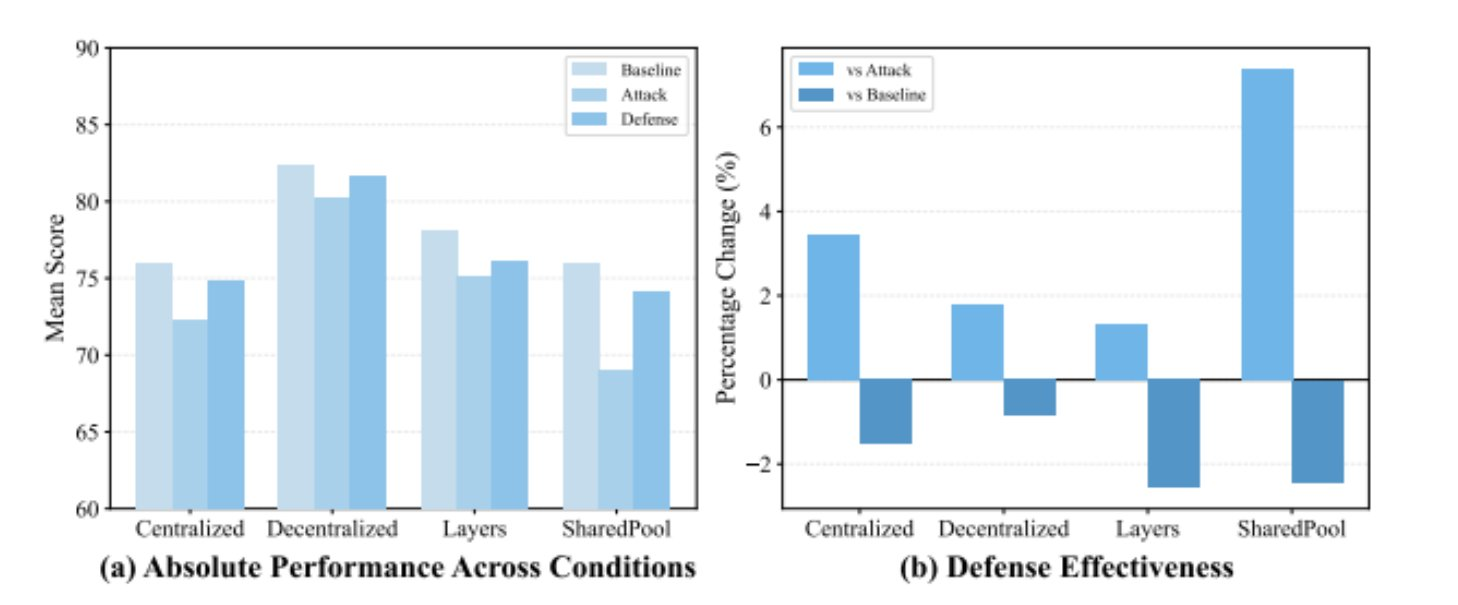
\includegraphics[width=0.85\textwidth]{images/medsentry_fig3}
\caption[MedSentry defence evaluation across MAS topologies]{Multi-agent system defence evaluation from Chen~et~al.~\cite{Chen2025MedSentry}.  (a)~Absolute performance scores across conditions (baseline, attack, defence) for four MAS topologies.  (b)~Percentage change showing defence effectiveness relative to the attack condition and the baseline.  The decentralised topology shows the highest absolute performance and resilience, while the centralised topology is most vulnerable to adversarial manipulation --- demonstrating that MAS topology is a primary determinant of clinical safety.}
\label{fig:medsentry}
\end{figure}

Complementing MedSentry's focus on adversarial resilience,
Wu~et~al.~\cite{Wu2024EHRFlow} addressed the distinct problem of operational
reliability with EHRFlow, published at the KDD 2024 Workshop on AI for Healthcare.
EHRFlow demonstrates automated, error-resilient EHR analysis through a four-agent
iterative pipeline: the Coder Agent translates natural language clinical queries into
executable Python analysis code; the Executor Agent runs the generated code; the
Debugger Agent automatically identifies execution errors and generates corrected code;
and the Summariser Agent converts raw computational outputs into clinically
interpretable narrative findings~\cite{Wu2024EHRFlow}.  EHRFlow achieved substantially
higher task completion rates than single-agent systems on clinical EHR analysis tasks
including cohort selection, longitudinal laboratory trend analysis, and outcome
prediction~\cite{Wu2024EHRFlow}.  The critical differentiating component was the
Debugger Agent's automated error-recovery loop, which prevented execution failures from
propagating downstream~\cite{Wu2024EHRFlow} --- a design pattern directly adopted in
this thesis.
